\chapter{Preliminaries and Subproblems}
\label{chap:location_nodes}

\section{Path Selection of Mobile elements}
It is known that controlled MULEs can increase a WSN's lifetime by saving energy. But the problem of planning an optimal path and job schedule is a hard problem in general, known as the Data MULE scheduling problem \cite{dms}. It has three components:
\begin{enumerate}
\item Path selection: which trajectory the data mule follows,
\item Speed control: how the data mule changes the speed while moving along the path,
\item and Job scheduling: from which sensor the data mule collects data at each time point.
\end{enumerate}
In this thesis we will focus only on Path selection of the MULEs.

Our path selection heuristic uses \emph{location nodes}. Since our MULEs need to communicate to  the sensors from 1-hop distance, we cover the sensor field with discs of radius equal to the range of the sensors. Ofcourse, we are approximating the communicable region of a sensor to a circular disc, and also assuming that the range of the MULE is greater than that of any sensor (we assume all the sensors are identical in communication range). The centres of these discs are called \emph{location nodes}.

\section{Geometric Disc Covering and Location Nodes}

In the interest of collecting data from sensors in one hop, we propose to cover the sensor field with circular discs of radius equal to the range of the sensors. The centers of these discs are going to be locations where MULEs will 
There are many \cite{gmdc} \cite{dudc} \cite{shifting} geometric disc covering algorithms and PTASs, any one of which can be used here. We, however used a greedy heuristic (GRD) for the implementation. Following are some heuristics that we tested on sample fields (in each of the following heuristics, assume that we have a set of discs $D$ such that any disc cover solution $D'$ is equivalent to a subset of $D$. By "picking a disc" we mean picking a disc from $D$.):
\begin{description}
\item[JGRD] Straightforward set cover heuristic \cite{jgreedy}. Pick the disc which covers the maximum number of uncovered sensors.
\item[GRD] We don't know whether this heuristic is known already or not. First sort the list of sensor positions according to their (x,y) position co-ordinates (first by x co-ordinate and then by y co-ordinate). Starting from the first sensor $s$ in the list, pick the disc which covers maximum number of uncovered sensors and covers $s$ too. Continue down this list until all the sensors are covered.
\item[SHFT] The shifting strategy from \cite{shifting}.
\item[SEL] For any sensor $s$, let $L$ be the set of discs covering it. Pick the disc which covers the least number of sensors.
\item[RND] Randomly pick discs until all the sensors are covered. Just for sake of comparision with other heuristics.
\end{description}

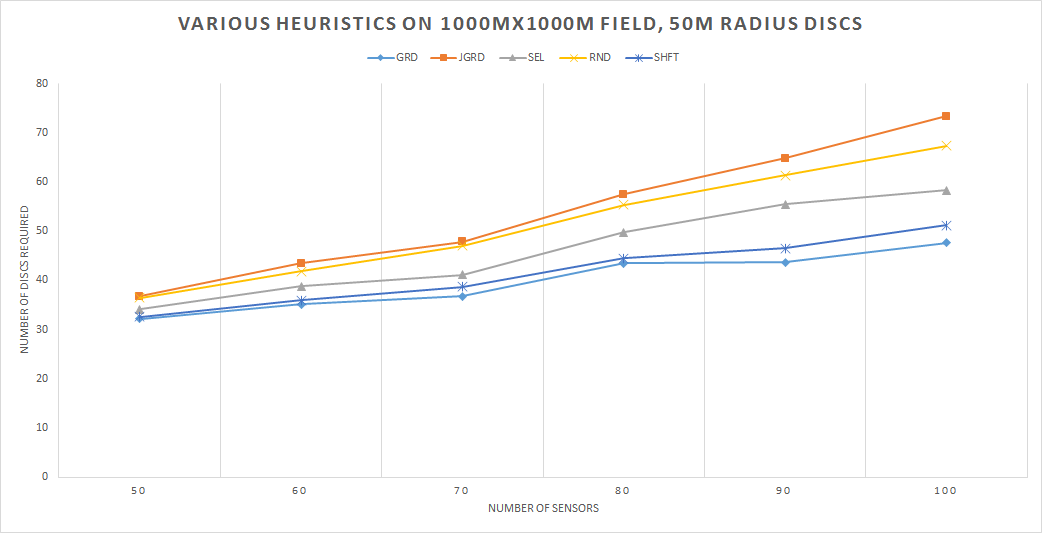
\includegraphics[width=15cm]{discs}